\section{Monitor Synchronization}

Communication between threads happens by sharing access to fields or object references. This can lead to thread interference and memory consistency errors. 

\begin{description}
  \item[Race Condition] 2 Threads try to update the same shared (on heap) resource. Outcome: either one of the threads can write, the other update gets lost.
  \item[Synchronization] restriction of concurrency to ensure overall correct / desired / deterministic behaviour.
  \item[Critical section] only one thread at a time can enter and execute this part of the code.
  \item[Atomicity] \verb|this.balance += amount| gets converted into three separate instructions. They will not be executed atomically.
\end{description}

\subsection{Java: Synchronized Methods with Monitor}

\begin{figure}
  \centering
  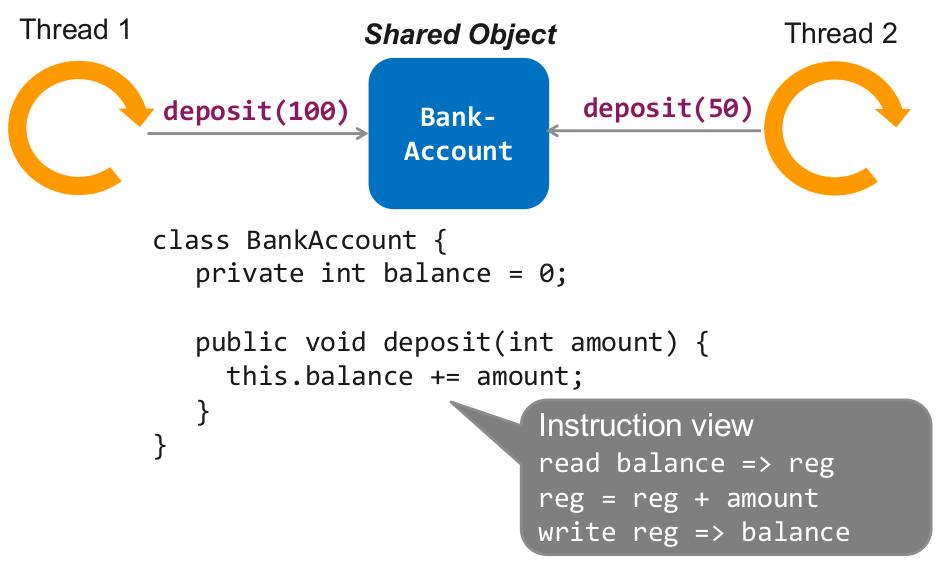
\includegraphics[width=10cm]{res/02-race-condition.png}
  \caption{Race Condition: Instruction View}
\end{figure}

\begin{description}
  \item[synchronized] This keyword in a method header marks it as a \textit{critical section}: only one thread can execute it at any moment. Impossible for two invocations of any synchronized method on the same object to interleave. After the execution of a synchronized method, the changed state on the object is guaranteed to be visible by all threads \textit{happens-before} relationship.
  \item[(Monitor-) Lock] Every object has a (Monitor-) Lock, which is acquired when any synchronized method is accessed. \verb|static| methods acquire the class objects lock which there is only one of.
  \item[synchronized statement block] Can be used inside a method. The object/instance whose lock should be used must be specified.
  \begin{verbatim}
    class BankAccount{
      private int balance = 0;
      public void deposit(int amount) {
        synchronized(this) {
          this.balance += amount;
        }
        System.out.println("Deposit done");
      }
    }
  \end{verbatim} 
  Exiting the synchronized block frees the lock: end, return statement, unhandled exception.
  \item[Internal mutual exclusion] Only one thread operates at a time. Every non-private method is synchronized.
  \item[Recursive Locks] Synchronized methods calling each other, lock will be freed by last release. 
\end{description} 

\subsection{Wait \& Signal Mechanism}
Two waiting rooms: outer to acquire monitor lock, inner to wait for condition to be fulfilled.\\

\noindent
Advantage: very powerful concept, object oriented. Disadvantage: Not always optimal: Inefficient with different waiting conditions, no fairness.

\begin{description}
  \item[wait()] temporarily releases the monitor lock so other threads can run. Used in while loop that checks for a condition.
  \item[notify] wake up one or all threads that are waiting. They will need to acquire access to the synchronized section again. \\
  \texttt{notify()} wakes one single thread. It is enough if two conditions are fulfilled:
  \begin{itemize}
    \item Uniform waiting condition (boolean): a change in the condition interests every waiting thread 
    \item One in one out: only a single waiting thread can continue
  \end{itemize}
  \texttt{notifyAll()} is for non-uniform waiting conditions. Every thread that is waiting re-checks their condition.
  \item[while-loop] Check should happen every time the thread has access to the Monitor, not just the first time. Thread execution continues from where it has left off.
  \item[Spurious Wakeup] thread wakes up out of a special reason, maybe woken by the OS. Makes while-loop for waiting important.
\end{description}

\subsubsection*{Details}
\begin{itemize}
  \item Monitor Lock is only freed on method end, not with the call to \texttt{notify/notifyAll}.
  \item \texttt{Wait}, \texttt{notify} and \texttt{notifyAll} can only be used inside a synchronized block.
\end{itemize}

\subsubsection*{Example} 
While loop is needed to check condition again after wakeup. 
\begin{verbatim}
class BankAccount {
  private int balance = 0;

  public synchronized void withdraw(int amount) throws InterruptedException {
    while (amount > balance) {
      wait();
    }
    balance -= amount;
  }
  public synchronized void deposit(int amount) {
    balance += amount;
    notifyAll();
  }
}
\end{verbatim}


